\section{Trasformata di Burrows-Wheeler posizionale}
\label{secpbwt}
Presentata nel 2014 da Richard Durbin la \textbf{Positional Burrows-Wheeler
  Transform (\textit{PBWT})} \cite{pbwt}, traducibile con \textit{trasformata di
  Burrows-Wheeler posizionale}, è una struttura efficiente per la memorizzazione
e l'interrogazione di pannelli di aplotipi.\\
Formalmente si considera un pannello $X$ di $M$ aplotipi $x_i$, $i=0,\ldots,
M-1$, su $N$ siti, indicizzati tramite $k=0,\ldots, N-1$, tale che tutti i siti
sono considerati biallelici. Da un punto di vista computazionale quest'ultima
assunzione comporta che il pannello $X$ è costruito sull'alfabeto $\Sigma
=\{0,1\}$, avendo quindi che:
\[x_i[k]=\{0,1\}\]
Si consideri che l'alfabeto è \textit{ordinato}, avendo che $0\prec 1$.\\
Prima di proseguire con la trattazione è bene fornire la descrizione di alcuni
formalismi utilizzati:
\begin{itemize}
  \item si denota, per una qualsiasi sequenza $s$, con $s[k_1,k_2)$ la
  \textbf{sottostringa} di $s$ che inizia alla colonna $k_1$ e termina alla colonna
  $k_2-1$
  \item date due sequenze $t$ e $s$, si definisce un \textbf{match} tra le due
  sequenze sse $s[k_1,k_2)=t[k_1,k_2)$, avendo che tale match inizia alla
  colonna $k_1$ e termina alla colonna $k_2-1$
  \item un match tra due sequenze $s$ e $t$, come definito al punto precedente,
  è definito \textbf{localmente massimale} sse non si ha alcuna estensione a
  destra o sinistra che comporti un ulteriore match, avendo quindi che:
  \[(k_1=0\lor s[k_1-1]\neq t[k_1-1])\land (k_2=N\lor s[k_2]\neq t[k_2] )\]
  \item comparando una sequenza $s$ ad un pannello di aplotipi $X$ si definisce
  che $s$ ha un \textbf{set-maximal match} con $x_i$, che inizia alla
  colonna $k_1$ e termina alla colonna $k_2-1$, sse tale match è
  \textit{localmente massimale} e non si ha alcun altro match di $s$ con un
  altro $x_j$ che include l'intervallo $[k_1,k_2)$
\end{itemize}
La costruzione di questa struttura dati si basa, ad ogni colonna $k$, sul
riordinamento lessicografico delle sequenze di aplotipi basato sull'ordinamento
inverso dei prefissi terminanti in colonna $k-1$. I valori presenti in colonna
$k$ dopo il riordinamento altro non sono che i valori che andranno a popolare la
cosiddetta \textbf{matrice PBWT}, che rappresenta la vera e propria
trasformata. Si noti che avere le sequenze 
ordinate in base ai prefissi invertiti alla $k$-esima colonna permette di
identificare i match con maggior facilità in quanto, ad ogni colonna, aplotipi
con suffisso comune (o prefisso comune in ordine inverso) saranno in posizioni
consecutive all'interno della trasformata.\\
La computazione di tutti i riordinamenti non presenta difficoltà dal punto di
vista computazionale in quanto, conoscendo l'ordinamento in colonna $k$, si può
derivare facilmente l'ordinamento in colonna $k+1$, studiando solo i valori alla
colonna precedente ed effettuando uno \textbf{step di radix sort}.\\
Più formalmente si denota con $a_k[i]=m$, con $m<M$, l'indice della sequenza
$x_m$ del pannello $X$ da cui deriva il prefisso $i$-esimo nell'ordine inverso
in colonna $k$. Si ottiene quindi che l'array $a_k$, detto \textbf{prefix
  array}, altro non è che una permutazione degli indici $0,\ldots,M-1$.
\begin{definizione}
  Dato un aplotipo $i$, appartenente al pannello $X$, e un indice di colonna
  $k$, si definisce il \textbf{prefix array} $a_k$ come una permutazione degli
  indici $0,\ldots, M-1$ tale che $a_k[i]=j$ sse $x_j$ è l'$i$-esimo aplotipo di
  $X$ nell'ordinamento inverso dei prefissi ottenuto alla colonna $k$.
\end{definizione}
Data questa definizione ne segue che la \textit{matrice PBWT} si ottiene
direttamente andando a vedere, per ogni colonna, gli indici del \textit{prefix
  array} e prendendo i valori del pannello $X$ secondo l'ordine espresso da
quell'array.\\ 
Per comodità di rappresentazione definiamo formalmente i valori della
\textit{matrice PBTW} con il seguente formalismo:
\[y_i^k[k]=x_{a_k[i]}[k]\]
avendo quindi che $y_i^k$ denota la sequenza $i$-esima secondo l'ordinamento
ottenuto per la colonna $k$. Possiamo quindi meglio spiegare perché risulti
semplice computare i vari \textit{prefix array}. Infatti, si ha
quindi che l'ordinamento degli elementi per $a_{k+1}$ è lo stesso degli elementi
per $a_k$, al più di ``guidare'' internamente il riordinamento tramite i valori
di $y_i^k[k]$, seguendo l'ordinamento dato dall'alfabeto. A breve, tramite un
esempio, si chiarirà meglio quanto detto.\\
\textbf{SPIEGARE MOLTO MEGLIO QUANTO DETTO}\\
Come anticipato prefissi simili saranno consecutivi nei riordinamenti fino alla
colonna $k$-esima risulta quindi utile tenere traccia della posizione iniziale
dei match tra prefissi vicini. Formalmente, dato $i>0$, si definisce il
$d_k[i]$ come il più piccolo $j$ tale che $y_i^k[j,k)=y_{i-1}^k[j,k)$. Ne segue
ovviamente che, se $y_i^k[k-1]\neq y_{i-1}^k[k-1]$, allora $d_k[i]=k$. Per
definizione, inoltre, $d_k[i]=k$ se $i=0$. L'array $d_k$ è detto
\textbf{divergence array}.
\begin{definizione}
  Si definisce \textbf{divergence array} l'array $d_k$ tale che $d_k[i]$ è
  l'indice colonna iniziale del match massimale a sinistra terminante in $k$ tra
  l'$i$-esimo aplotipo e il suo precedente nell'ordinamento ottenuto alla
  colonna $k$-esima.
\end{definizione}
Si può quindi dimostrare che l'inizio di qualsiasi match massimale terminante in
colonna $k$ tra qualsiasi $y_i^k$ e $y_j^k$, con $i<j$, è calcolabile facilmente
avendo che è dato da:
\[\max_{i<m\leq j}d_k[m]\]
Si noti che al posto del \textbf{divergence array} si può usare anche una
variante del \textbf{Longest Common Prefix (\textit{LCP}) array}, denotato
$l_k$, che, anziché 
memorizzare l'indice d'inizio del match massimale a sinistra da due aplotipi
consecutivi nell'ordinamento ottenuto alla colonna $k$-esima, tiene traccia
della lunghezza di tale match. Formalmente si ha che $l_k[i]=k-d_k[i]$. \\ 
\textbf{FORSE SERVE DEFINIZIONE FORMALE}.\\
Fatte queste premesse possiamo quindi fornire una definizione formale di
\textbf{PBWT}.
\begin{definizione}
  Dato $X=\{x_1,x_2,\ldots,x_M\}$ un insieme/pannello di $M$ aplotipi con $N$
  siti, la \textbf{PBWT} di $X$ è una collezione di $N+1$ coppie di array
  $(a_k,d_k)$, con $0\leq k\leq N$, dove ogni $a_k$ è detto \textbf{prefix
    array} e ogni $d_k$ è detto \textbf{divergence array}. 
\end{definizione}
L'algoritmo per la costruzione di $a_{k+1}$ e $d_{k+1}$ a partire da $a_k$ e
$d_k$ è disponibile all'algoritmo \ref{algo:durbin1}.\\
Ai fini della trattazione dell'algoritmo di match con un'aplotipo esterno
ricordiamo un'ulteriore definizione.
\begin{definizione}
  Definiamo $\alpha_k$ come l'inverso della permutazione data dal \textbf{prefix
    array} $a_k$, avendo che:
  \[\alpha_k[i]=j \iff a_k[j]=i\]
\end{definizione}
\begin{esempio}
  \label{es:pbwt1}
  Vediamo quindi un esempio chiarificatore.\\
  Si assuma il seguente pannello $X$:
  \begin{table}[H]
    \centering
    \footnotesize
    \begin{tabular}{c|ccccccccccccccc}
      X & 00 & 01 & 02 & 03 & 04 & 05 & 06 & 07 & 08 & 09 & 10 & 11 & 12 & 13
      & 14 \\
      \hline
      00 & 1 & 0 & 0 & 1 & 0 & 0 & 0 & 0 & 0 & 0 & 0 & 1 & 1 & 0 & 1 \\
      01 & 1 & 0 & 0 & 1 & 1 & 0 & 0 & 1 & 0 & 0 & 0 & 0 & 0 & 1 & 1 \\
      02 & 1 & 0 & 0 & 1 & 1 & 0 & 0 & 1 & 0 & 0 & 0 & 1 & 0 & 0 & 1 \\
      03 & 1 & 0 & 0 & 1 & 1 & 0 & 0 & 1 & 0 & 0 & 0 & 1 & 0 & 0 & 1 \\
      04 & 0 & 1 & 0 & 1 & 0 & 1 & 0 & 0 & 0 & 0 & 0 & 1 & 0 & 0 & 1 \\
      05 & 0 & 1 & 0 & 1 & 0 & 1 & 0 & 0 & 0 & 0 & 0 & 1 & 0 & 0 & 1 \\
      06 & 0 & 1 & 0 & 1 & 0 & 1 & 0 & 0 & 0 & 0 & 0 & 1 & 0 & 0 & 1 \\
      07 & 0 & 1 & 0 & 1 & 0 & 1 & 0 & 0 & 0 & 0 & 0 & 0 & 1 & 0 & 1 \\
      08 & 0 & 1 & 0 & 0 & 1 & 0 & 0 & 0 & 0 & 1 & 1 & 1 & 0 & 0 & 1 \\
      09 & 0 & 1 & 0 & 1 & 0 & 0 & 0 & 0 & 1 & 0 & 0 & 0 & 0 & 1 & 1 \\
      10 & 0 & 1 & 0 & 1 & 0 & 0 & 0 & 0 & 1 & 0 & 0 & 0 & 0 & 1 & 1 \\
      11 & 0 & 1 & 0 & 0 & 1 & 0 & 0 & 0 & 0 & 0 & 1 & 1 & 0 & 0 & 0 \\
      12 & 0 & 1 & 0 & 0 & 1 & 0 & 0 & 0 & 1 & 0 & 1 & 1 & 0 & 0 & 1 \\
      13 & 0 & 1 & 0 & 0 & 1 & 0 & 0 & 0 & 1 & 0 & 1 & 1 & 0 & 0 & 1 \\
      14 & 0 & 1 & 0 & 0 & 0 & 0 & 0 & 0 & 1 & 0 & 0 & 0 & 1 & 0 & 1 \\
      15 & 0 & 1 & 0 & 0 & 0 & 0 & 0 & 0 & 1 & 0 & 0 & 0 & 1 & 0 & 1 \\
      16 & 0 & 1 & 0 & 1 & 0 & 0 & 0 & 0 & 0 & 0 & 0 & 1 & 1 & 0 & 1 \\
      17 & 1 & 1 & 0 & 0 & 0 & 1 & 0 & 0 & 0 & 0 & 0 & 1 & 1 & 0 & 1 \\
      18 & 0 & 1 & 1 & 0 & 1 & 0 & 0 & 0 & 0 & 0 & 0 & 1 & 0 & 0 & 1 \\
      19 & 0 & 1 & 1 & 0 & 1 & 0 & 1 & 0 & 0 & 0 & 0 & 0 & 1 & 0 & 1 
    \end{tabular}
  \end{table}
  Volendo calcolare $y^6$ riordiniamo il pannello con l'ordine inverso alla
  quinta colonna e $y^6$ altro non è che la sesta colonna del pannello
  riordinato, $a_6$ la colonna degli indici e $d_6$ la colonna iniziale in cui
  terminano le sottolineature:  
  \begin{figure}[H]
    \centering
    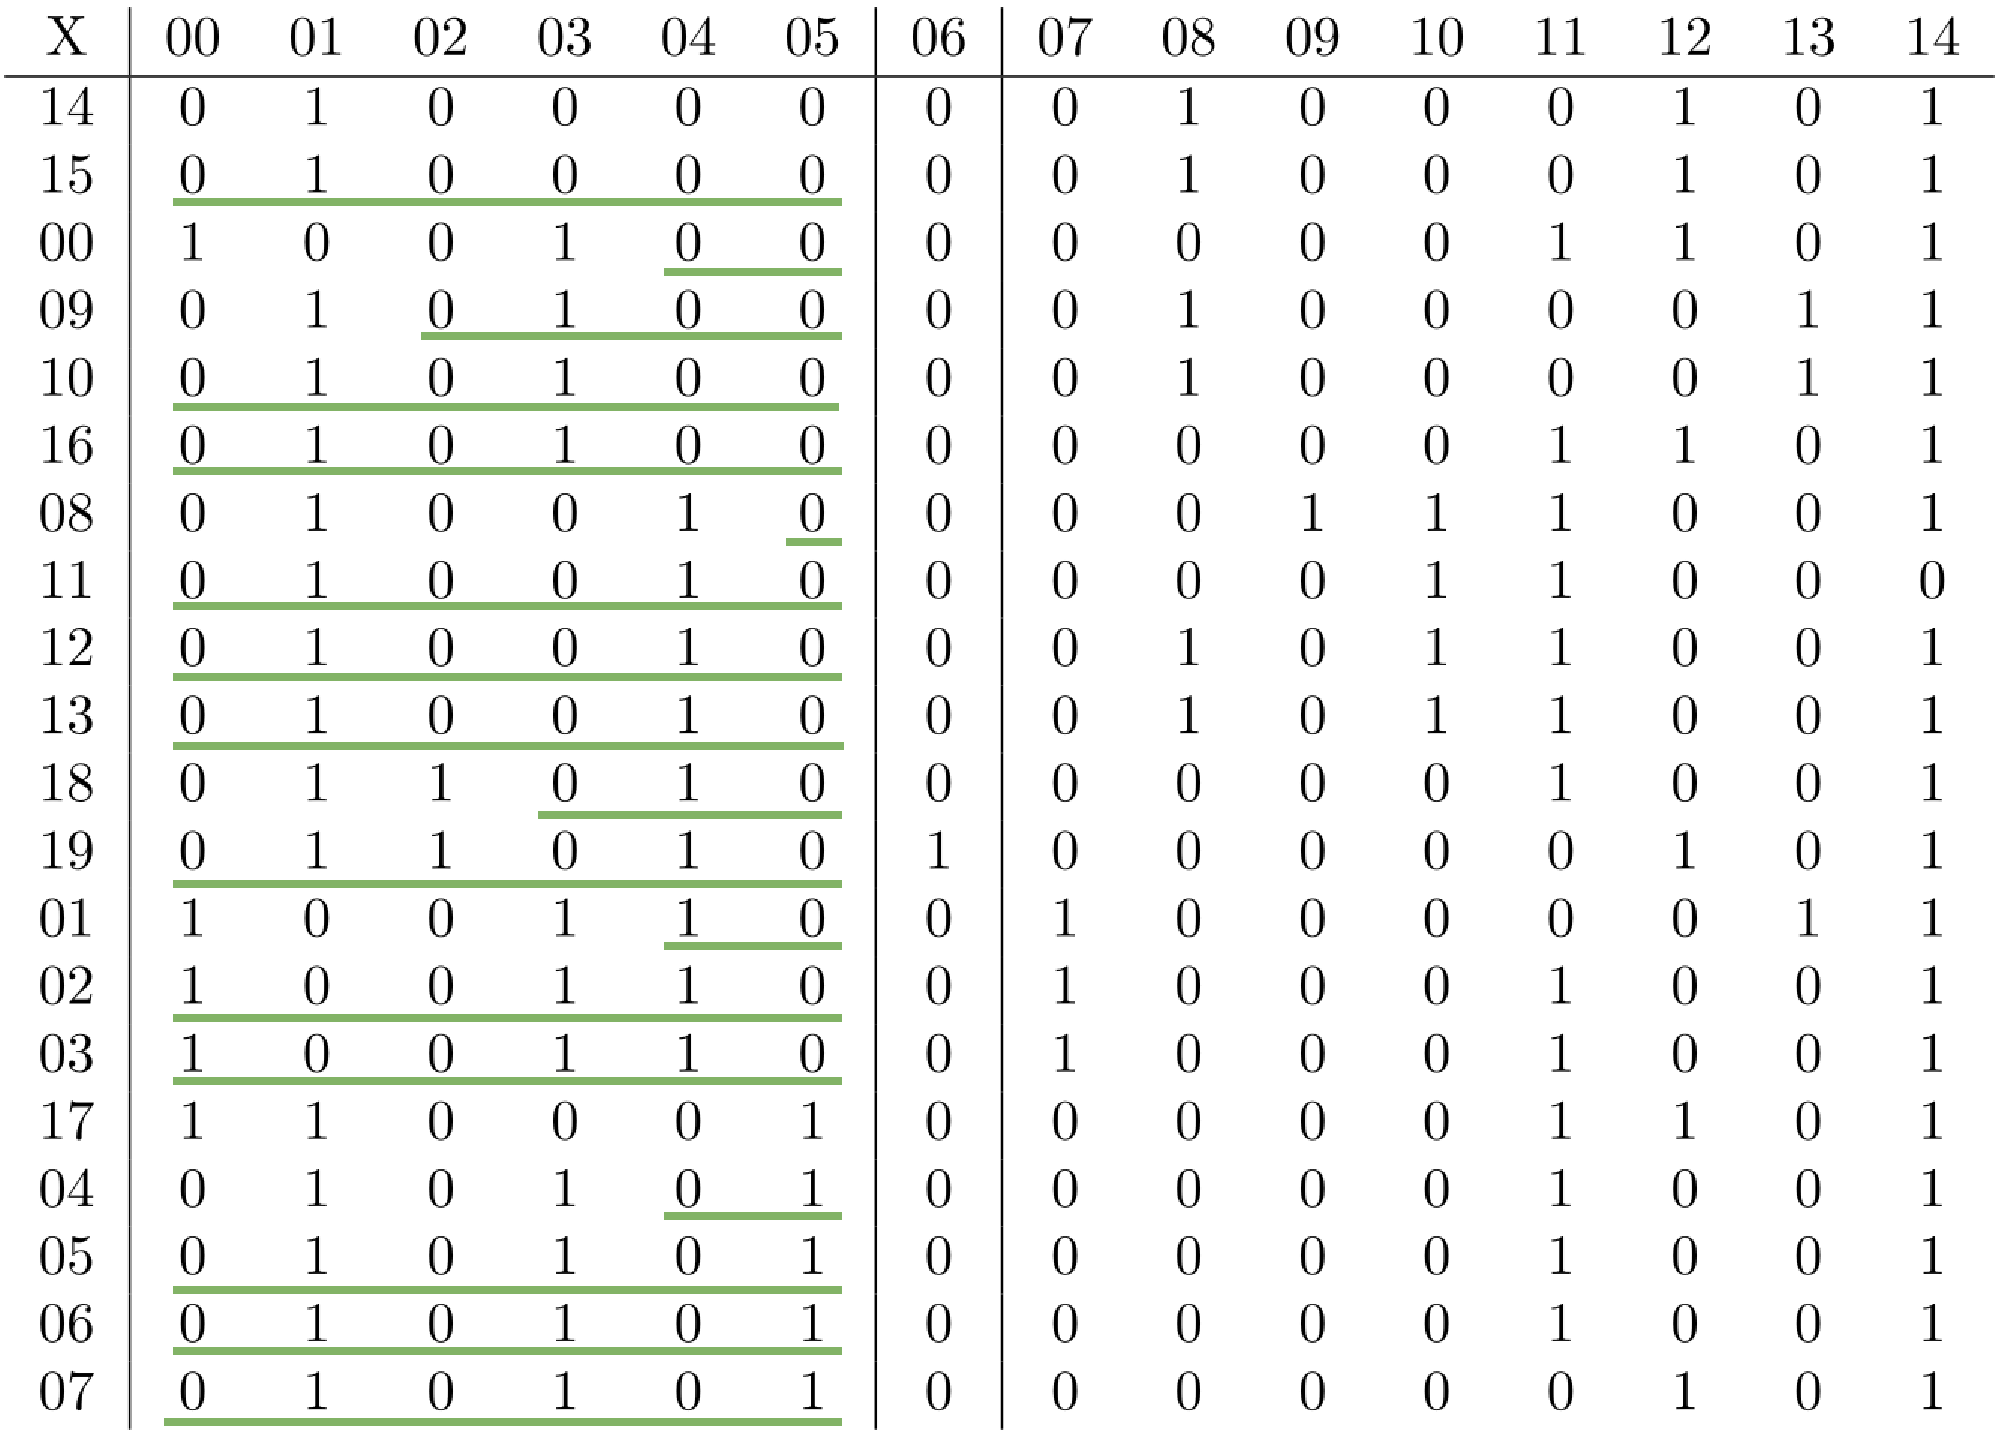
\includegraphics[scale = 0.365]{img/matrix1.pdf}
  \end{figure}
  Ottenendo quindi:
  \[a_6=[14,15,0,9,10,16,8,11,12,13,18,19,1,2,3,17,4,5,6,7]\]
  \[\alpha_6=[2,12,13,14,16,17,18,19,6,3,4,7,8,9,0,1,5,15,10,11]\]
  \[d_6=[6,0,4,2,0,0,5,0,0,0,3,0,4,0,0,6,4,0,0,0]\]
  \[l_6=[0,6,2,4,6,6,1,6,6,6,3,6,2,6,6,0,2,6,6,6]\]
  Nel complesso, permutando con tutti i vari \textit{prefix array}, si
  otterrebbe la seguente \textbf{matrice PBTW}:
  \begin{table}[H]
  \centering
  \footnotesize
  \begin{tabular}{c|ccccccccccccccc}
    X & 00 & 01 & 02 & 03 & 04 & 05 & 06 & 07 & 08 & 09 & 10 & 11 & 12 & 13
    & 14 \\
    \hline
    00 & 1 & 1 & 0 & 1 & 1 & 0 & 0 & 0 & 1 & 0 & 0 & 1 & 1 & 1 & 1 \\
    01 & 1 & 1 & 0 & 1 & 1 & 0 & 0 & 0 & 1 & 0 & 0 & 1 & 1 & 1 & 1 \\
    02 & 1 & 1 & 0 & 1 & 1 & 1 & 0 & 0 & 0 & 1 & 1 & 1 & 0 & 1 & 1 \\
    03 & 1 & 1 & 0 & 1 & 1 & 0 & 0 & 0 & 1 & 0 & 0 & 1 & 1 & 0 & 1 \\
    04 & 0 & 1 & 0 & 1 & 0 & 1 & 0 & 0 & 1 & 0 & 0 & 1 & 1 & 0 & 1 \\
    05 & 0 & 1 & 0 & 1 & 0 & 1 & 0 & 0 & 0 & 0 & 0 & 1 & 0 & 0 & 1 \\
    06 & 0 & 1 & 0 & 1 & 0 & 1 & 0 & 0 & 0 & 0 & 0 & 1 & 0 & 0 & 0 \\
    07 & 0 & 1 & 0 & 1 & 1 & 1 & 0 & 0 & 0 & 0 & 0 & 0 & 1 & 0 & 1 \\
    08 & 0 & 1 & 0 & 0 & 1 & 0 & 0 & 0 & 1 & 0 & 0 & 0 & 1 & 0 & 1 \\
    09 & 0 & 1 & 0 & 1 & 0 & 0 & 0 & 0 & 1 & 0 & 0 & 0 & 0 & 0 & 1 \\
    10 & 0 & 1 & 0 & 1 & 1 & 0 & 0 & 0 & 0 & 0 & 0 & 1 & 1 & 0 & 1 \\
    11 & 0 & 1 & 0 & 0 & 1 & 0 & 1 & 1 & 0 & 0 & 0 & 1 & 0 & 0 & 1 \\
    12 & 0 & 1 & 0 & 0 & 1 & 0 & 0 & 1 & 0 & 0 & 0 & 0 & 0 & 0 & 1 \\
    13 & 0 & 1 & 0 & 0 & 0 & 0 & 0 & 1 & 0 & 0 & 0 & 0 & 0 & 0 & 1 \\
    14 & 0 & 1 & 0 & 0 & 0 & 0 & 0 & 0 & 0 & 0 & 0 & 0 & 0 & 0 & 1 \\
    15 & 0 & 0 & 0 & 0 & 0 & 0 & 0 & 0 & 0 & 0 & 0 & 0 & 0 & 0 & 1 \\
    16 & 0 & 0 & 0 & 1 & 0 & 0 & 0 & 0 & 0 & 0 & 0 & 1 & 0 & 0 & 1 \\
    17 & 1 & 0 & 1 & 0 & 0 & 0 & 0 & 0 & 0 & 0 & 1 & 1 & 0 & 0 & 1 \\
    18 & 0 & 0 & 1 & 0 & 0 & 0 & 0 & 0 & 0 & 0 & 1 & 1 & 0 & 0 & 1 \\ 
    19 & 0 & 1 & 0 & 0 & 0 & 0 & 0 & 0 & 0 & 0 & 1 & 1 & 0 & 0 & 1
  \end{tabular}
\end{table}
\end{esempio}
\subsection{Match con aplotipo esterno}
Durbin, nel suo articolo, propone diversi algoritmi, ad esempio per il calcolo
di match interni ad $X$ più lunghi di una lunghezza minima $L$ o per la ricerca
di tutti i \textit{set-maximal match} interni ad $X$ in tempo lineare. Di
interesse per questa tesi è però il cosiddetto \textit{algoritmo 5}, quello che
si propone di trovare tutti i \textit{set-maximal match} tra il panello $X$ e un
aplotipo esterno $z$, assumendo che $|z|=M$.\\
L'idea dietro l'algoritmo è quella di usare tre indici: $e_k$, $f_k$ e
$g_k$. Nel dettaglio $e_k$ tiene traccia dell'inizio del più lungo match,
terminante in colonna $k$, tra $z$ e un qualche $y_i^k$. L'intervallo
$[f_k,g_k)\subseteq[0,\ldots,M)$ invece identifica il sotto-intervallo di
$a_k$ contenente gli indici degli aplotipi appartenetenti a tale match.
\begin{definizione}
  Dato un pannello $X$, con $M$ aplotipi/righe e $N$ colonne, e un aplotipo
  query $z$, tale che $|z|=n$, si definisce un \textbf{Set-Maximal Exact Matches
    (\textit{SMEM})}, iniziante in colonna $e_k$ e terminante il colonna
  $k$, tra 
  la query $z$ e le righe del pannello indicizzate dai valori compresi
  nell'intervallo $[f_k,g_k)$ in $a_k$ sse:
  \[z[e_k,k)=y_i^k[e_k,k)\land z[e_k-1]\neq y_i^k[e_k-1], \forall i\mbox{
      t.c. }f_k\leq i < g_k\]
  Si noti che $g_k=M$ sse $y_{M-1}^k$ appartiene alle sequenze per cui si ha tale
  match più lungo.\\
\end{definizione}

Bisogna quindi capire come aggiornare $e_k$, $f_k$ e $g_k$ passando dalla
colonna $k$ alla colonna $k+1$. L'idea è quella per cui, avendo
$f_{k+1}<g_{k+1}$ allora sicuramente ho ancora delle righe che presentano un
match che parte da $e_k=e_{k+1}$ e termina in $k$ che può essere esteso in
$k+1$. In caso contrario, avendo $f_{k+1}=g_{k+1}$, non si hanno match
estendibili e quindi si può concludere che quelli terminanti in colonna $k$
erano match massimali, dovendo poi aggiornare $e_{k+1}$ ottenedo i relativi
$f_{k+1}$ e $g_{k+1}$. Bisogna quindi capire come funzioni la
variante dell'\textbf{LF-mapping}, guidato dal carattere corrente dell'aplotipo
query, all'interno della \textbf{PBWT}, per ottenere $f_{k+1}$ e $g_{k+1}$ a
partire da $f_k$ e $g_k$ (e di conseguenza $e_{k+1}$).\\ 
Per effettuare il mapping abbiamo bisogno di tre componenti:
\begin{enumerate}
  \item l'array $c$ tale per cui $c[k]=j$ sse la colonna $k$ contiene $j$
  occorrenze di 0
  \item l'array $u_k$ tale per cui, alla colonna $k$-esima, $u_k[i]=j$ sse $j$ è
  il numero di occorrenze di 0 prima dell'indice $i$ nella colonna $k$
  \item l'array $v_k$ tale per cui, alla colonna $k$-esima, $v_k[i]=j$ sse $j$ è
  il numero di occorrenze di 1 prima dell'indice $i$ nella colonna $k$ 
\end{enumerate}
Tali valori possono essere computati e memorizzati in fase di costruzione della
\textbf{PBWT}, come visibile direttamente nell'algoritmo \ref{algo:durbin1} per
quanto riguarda $u$ e $v$, avendone già la computazione. Per quanto riguarda $c$
si ha che potrebbe essere banalmente calcolato anch'esso in fase di costruzione
della \textbf{PBWT}, tenendo ogni volta traccia del numero di 0 incontrati
nella colonna $k$-esima.\\
Sfruttando i valori di questi 3 array possiamo quindi effettuare il mapping,
definito per comodità da una funzione, rappresentabile in pseudocodice come
nell'algoritmo \ref{algo:lf}:
\[w_k:\{0,\ldots,M\}\times\Sigma\to \{0,\ldots,M\}\]
tale per cui:
\[w_k(i,\sigma)=
  \begin{cases}
    u_k[i]&\mbox{ se }\sigma=0\\
    v_k[i]+c[k]&\mbox{ se }\sigma=1
  \end{cases}
\]
Infatti, come confermato anche dall'algoritmo di costruzione stesso, si ha che:
\[a_{k+1}\left[w_k\left(i,y_i^k[k]\right)\right]=a_k[i]\]
\begin{esempio}
  Vediamo un piccolo esempio chiarificatore, riprendendo il precedente.\\
  Per praticità riporta che:
  \[a_5=[14,15,17,0,4,5,6,7,9,10,16,8,11,12,13,18,19,1,2,3]\]
  \[\alpha_5=[3,17,18,19,4,5,6,7,11,8,9,12,13,14,0,1,10,2,15,16]\]
  \[a_6=[14,15,0,9,10,16,8,11,12,13,18,19,1,2,3,17,4,5,6,7]\]
  \[\alpha_6=[2,12,13,14,16,17,18,19,6,3,4,7,8,9,0,1,5,15,10,11]\]
  Si ha quindi, ad esempio, con $k=5$ e $i=2$, che:
  \[a_{6}\left[w_5\left(2,y_2^5[5]\right)\right]=a_5[2]\]
  Avendo:
  \[w_5\left(2,y_2^5[5]\right)=w_5\left(2,1\right)=v_5[2]+c[5]=0+15=15\]
  Si ha che:
  \[a_{6}[15]=17=a_5[2]\]
\end{esempio}
Ai fini dell'algoritmo serve però il ``passaggio inverso'' rispetto a quello
indicato da questa equazione, ovvero passare dalla colonna $k$ alla colonna
$k+1$. Quindi, pensando alla permutazione inversa del \textbf{prefix array}, si
ha che:
\[\alpha_{k+1}[i]=w_k(\alpha_k[i],x_i[k])\]
\begin{esempio}
  Si riprendono i dati dell'esempio precedente e si vuole calcolare, sempre con
  $k=5$ e $i=2$:
  \[\alpha_{6}[2]=w_5(\alpha_5[2],x_2[5])=w_5(18,0)=13\]
  Come volevasi dimostrare.
\end{esempio}
L'ultima equazione ci suggerisce quindi che l'LF-mapping sopra definito
consente il corretto aggiornamento di $f_k$ e $g_k$.
Definendo quindi:
\[f_{k+1}=w_k(f,z[k])\]
si ha che $f_{k+1}$ sarà l'indice, in $a_{k+1}$, della prima sequenza $y_j^k$,
con $j\geq f$, per la quale $y_j^k[k]=z[k]$. Analogamente si ha anche:
\[g_{k+1}=w_k(g,z[k])\]
Si hanno quindi, dopo il calcolo di $f_{k+1}$ e $g_{k+1}$ due possibili casi:
\begin{enumerate}
  \item si ha che $f_{k+1}<g_{k+1}$, quindi si hanno ancora match che partono da
  $e_k$ e terminano in $k$ che si estendono anche in $k+1$. In tal caso quindi
  $e_{k+1}=e_k$
  \item si ha che $f_{k+1}=g_{k+1}$, quindi non si hanno match che partono da
  $e_k$ e terminano in $k$ che sono anche estendibili in $k+1$. Bisogna quindi
  annotare i match terminanti in $k$, nell'intervallo $[f_k,g_k)$ su $a_k$,
  e poi calcolare i nuovi $e_k$, $f_k$ e $g_k$. La chiave per questo calcolo è
  che, virtualmente, l'aplotipo $z$ si trova o  subito prima del blocco di
  aplotipi $[f_k,g_k)$ in colonna $k$, secondo l'ordinamento dato dalla medesima
  colonna, o subito dopo. Si ha quindi che, essendo nell'ordinamento o subito
  prima di $f_{k}$ o subito dopo $g_k$:
  \[y_{f_{k+1}-1}^{k+1}<z<y_{f_{k+1}}^{k+1}\]
  Diventa quindi possibile inferire che:
  \[e_{k+1}\leq d_{k+1}[f_{k+1}]\]
  Si considera quindi, come punto di partenza $e_{k+1}=d_{k+1}[f_{k+1}]-1$,
  studiando di conseguenza $z[e_{k+1}]$, avendo due casi possibili:
  \begin{enumerate}
    \item se tale valore è 0 allora, per l'ordinamento, $z$ ha un match migliore
    con $y_{f_{k+1}-1}^{k+1}$ rispetto che con $y_{f_{k+1}}^{k+1}$. Si aggiorna
    quindi $e_{k+1}$, decrementandolo, fino a che si ha match tra $z[e_{k+1}-1]$
    e $y_{f_{k+1}-1}^{k+1}[e_{k+1}-1]$. Infine si decrementa $f_{k+1}$ fino a
    che $d_{k+1}[f_{k+1}]\leq e_{k+1}$, trovando quelle righe per il quale il
    \textbf{divergence array} non supera il valore di $e_{k+1}$. Si ottengono in
    tal modo le sequenze, nel riordinamento in $k+1$, che hanno un match da
    $e_{k+1}$ a $k+1$. Invece $g_{k+1}$ resta fisso
    \item se tale valore è 1 allora, per l'ordinamento, $z$ ha un match migliore
    con $y_{f_{k+1}}^{k+1}$ rispetto che con $y_{f_{k+1}-1}^{k+1}$. Si aggiorna
    quindi $e_{k+1}$, decrementandolo, fino a che si ha match tra $z[e_{k+1}-1]$
    e $y_{f_{k+1}-1}^{k+1}[e_{k+1}-1]$. Infine si incrementa $g_{k+1}$ fino a
    che $d_{k+1}[g_{k+1}]\leq e_{k+1}$, per lo stesso ragionamento del caso
    precedente. Invece $f_{k+1}$ resta fisso 
  \end{enumerate}
\end{enumerate}
Si noti inoltre che, a livello di inizializzazione, si hanno:
\[f_0=g_0=e_0=0\]
Quindi il primo step sarà già un caso in cui $f_k=g_k$ qualora $x_0[0]=y_0^0\neq
z[0]$. 
\begin{esempio}
  \label{es:algo5}
  Mostrare un esempio completo di esecuzione richiederebbe troppo tempo quindi
  ci si limita a mostrare cosa succede nel caso in cui, ad un certo punto
  dell'esecuzione si hanno $f_{k+1}=g_{k+1}$.\\
  Si assuma il pannello e la \textit{matrice PBWT} visti all'esempio
  \ref{es:pbwt1} con una query $z$. Nel complesso si identificherebbero i
  seguenti match:
  \begin{figure}[H]
    \centering
    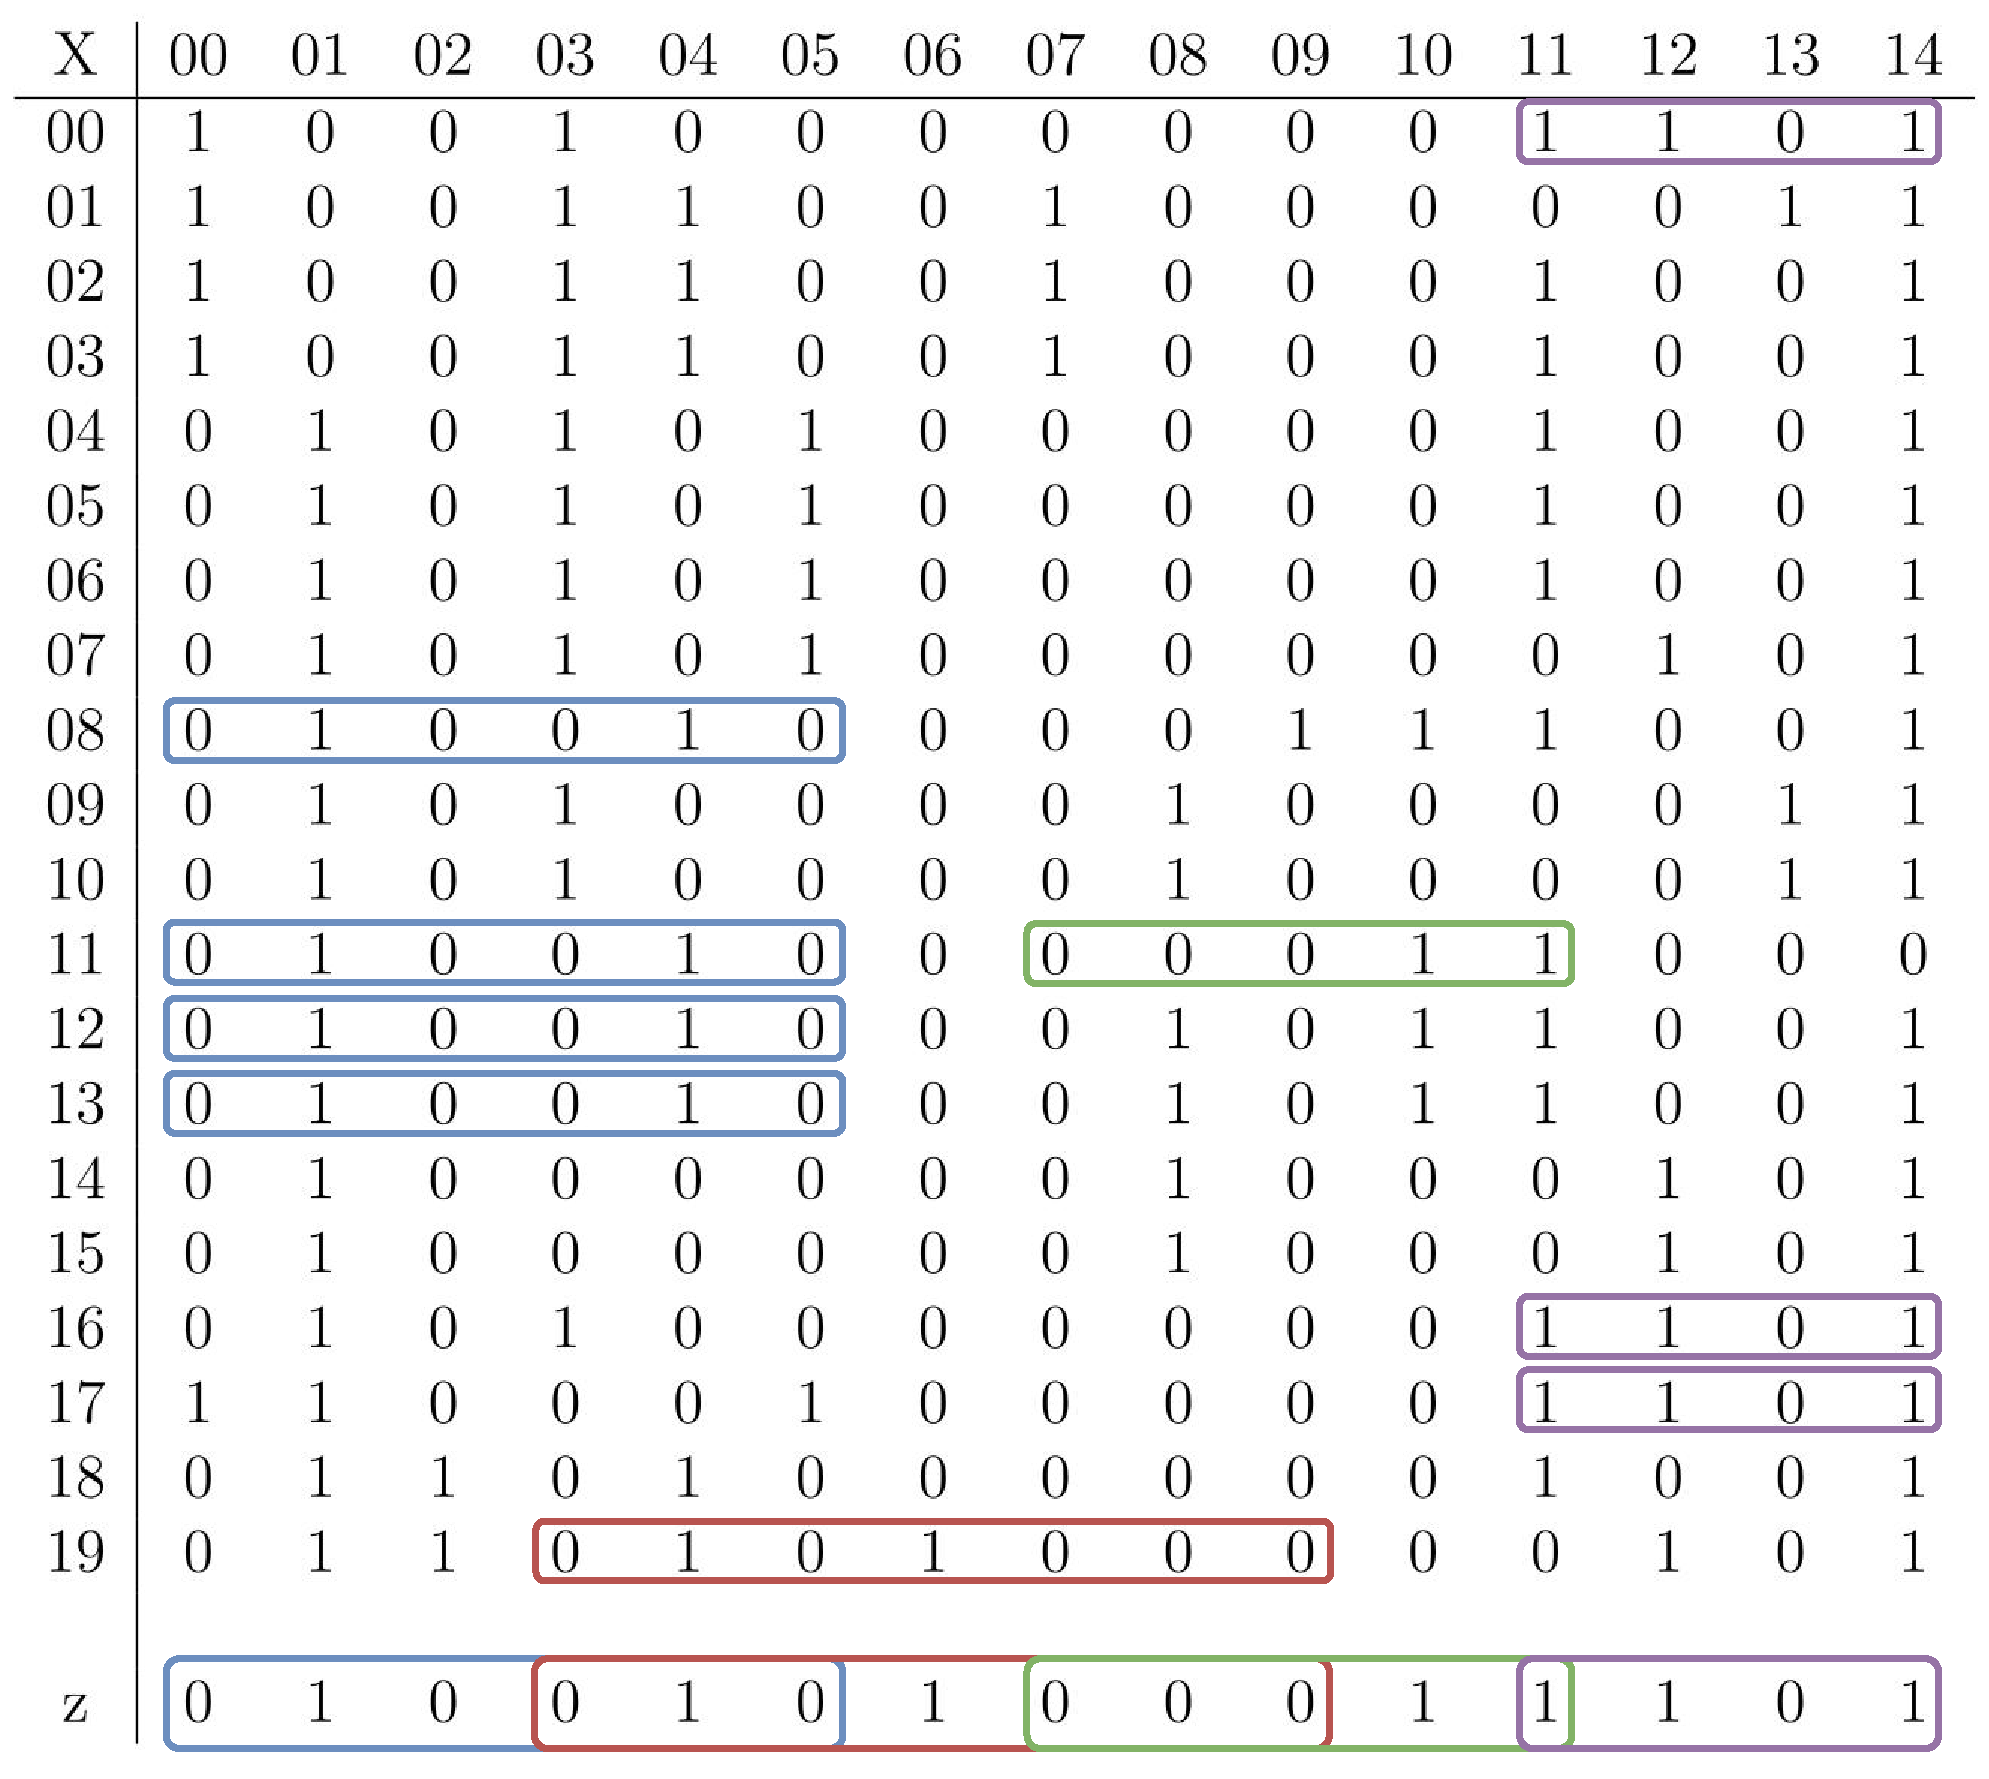
\includegraphics[scale = 0.365]{img/pbwtmatch.pdf}
  \end{figure}
  Si assuma di essere in colonna $k=6$, avendo, dopo i calcoli fatti in colonna
  $k=5$: 
  \begin{itemize}
    \item $f_6=6$
    \item $g_6=10$
    \item $e_6=0$
  \end{itemize}
  Avendo quindi che, a partire dalla colonne $0$ fino alla colonna $6-1=5$ si
  hanno le righe nel range $[6,10)$ di $a_{5}$ che matchano con $z[0,5]$.\\
  Bisogna quindi aggiornare $f$ e $g$. Si assuma che $z[6]=1$ e che:
  \[y^6=00000000000100000000,\,\,\,c[6]=19\]
  Si calcolano quindi:
  \[f_7=w_6(6,1)=v_6[6]+c[6]=0+19=19\]
  \[g_7=w_6(10,1)=v_6[10]+c[6]=0+19=19\]
  Avendo quindi $f_7=g_7$ si procede, in primis, annotando i match terminanti in
  $k_5$.\\
  Seguendo l'algoritmo si ha quindi un primo aggiornamento di $e_{k+1}$, che
  viene inizializzato a, avendo in memoria $d_7$ con random access in tempo
  costante: 
  \[e_7=d_7[19]-1=7-1=6\]
  Questo viene fatto in quanto, come detto, l'aplotipo $z$ si trova o subito
  prima del blocco di aplotipi $[f_k,g_k)$.\\
  Essendo inoltre $z[e_7]=z[6]=1$ si procede aggiornando $g$ e tenendo fermo
  $f$, avendo che, essendo $z[6]=1$, gli aplotipi che matchano seguiranno nel
  mapping tramite il simbolo $\sigma=1$. Si procede quindi inizializzando il
  nuovo $g$:
  \[g_7=f_7+1=20\]
  ricordando che $g$ può ``superare'' le dimensioni del pannello essendo
  escluso in $[f_k,g_k)$.\\
  A questo punto si segue la linea specificata da $f_7$ in $a_7$ a ritroso,
  partendo da $e_7-1$, fino a che si hanno match con $z$, aggiornando così il
  valore di $e_7$.\\
  In questo caso non si hanno altre operazioni, in quanto $g_7=M$ ma, qualora
  non lo fosse stato, si sarebbe incrementato $g_7$ fino a che il corrispondente
  $d_7[g_7]$ sarebbe stato minore o uguale di $e_7$, identificando tutte le
  nuove righe che hanno un match da $e_7$ a $k=6$ con $z$.
\end{esempio}
\textbf{SISTEMARE ESEMPIO E CAPIRE SE METTERE LE IMMAGINI}\\
L'algoritmo 5 è visualizzabile all'algoritmo \ref{algo:dur5} e, secondo i
calcoli di Durbin, ha complessità $\mathcal{O}(NM)$, in quanto si ritiene che il
numero di accessi ai loop interni sia limitato dalla costante rappresentante il
numero di match, $c$. Nonostante ciò tale complessità temporale è ancora in
corso di studio in quanto si hanno in letteratura evidenze della sua non
correttezza. Un esempio è il paper di Naseri \cite{dpbwt}, dove si afferma che
l'intuizione per cui tale costante $c$ limiti superiormente gli accessi ai loop
innestati sia falsa. Si noti che nell'articolo non viene però precisata una
nuova misura per la complessità dell'algoritmo.
\textbf{VERIFICARE ULTIMA FRASE (MA ANCHE TUTTO IL RESTO CHE VA SCRITTO MEGLIO)}
\begin{algorithm}
  \begin{algorithmic}   
    \Function{Find\_Set\_Maximal\_Matches\_From\_Z}{$z$}
    \For {$k\gets 0$ \textbf{to} $N$}
    \State $e,f,g\gets \mbox{\textit{Update\_Z\_Matches}}(k, z, e, f, g)$
    \EndFor
    \EndFunction    
    \Function{Update\_Z\_Matches}{$k, z, e, f, g$}
    \State $f'\gets w(k, f, z[k])$
    \State $g'\gets w(k, g, z[k])$
    \If{$f'<g'$}
    \Comment\textit{{se $k$ è $N-1$ match da $e_k$ a $N-1$}}
    \State $e'\gets e_k$
    \Else
    \Comment{\textit{match da $e_k$ a $k$}}
    \State $e'\gets d_{k+1}[f']-1$
    \If{$z[e']=0$ \textbf{and} $f'>0$}
    \State $f'\gets g'-1$
    \State \textbf{while} $z[e'-1]=y_{f'}^{k+1}[e'-1]$ \textbf{do} $e'\gets
    e'-1$
    \State \textbf{while} $d_{k+1}[f']\leq e'$ \textbf{do} $f'\gets f'-1$
    \Else
    \State $g'\gets f'+1$
    \State \textbf{while} $z[e'-1]=y_{f'}^{k+1}[e'-1]$ \textbf{do}  $e'\gets
    e'-1$ 
    \State \textbf{while} $g'<M$ \textbf{and} $d_{k+1}[g']\leq e'$ \textbf{do}
    $g'\gets g'+1$ 
    \EndIf
    \EndIf
    \State \textbf{return} $e',f',g'$
    \EndFunction
  \end{algorithmic}
  \caption{Algoritmo 5 di Durbin.}
  \label{algo:dur5}
\end{algorithm}
\subsubsection{Limiti spaziali}
Bisogna affrontare la tematica della complessità in spazio di tale
algoritmo. Ipotizzando di non ricalcolare colonna per colonna tutti i dati
necessari (comportando un'incremento dal punto di vista temporale).\\
Ricapitolando, per poter eseguire l'algoritmo 5, si necessita di avere in
memoria, con \textit{random access} in tempo costante:
\begin{itemize}
  \item il \textbf{pannello} $X$, di dimensione $NM$
  \item il \textbf{prefix array} $a_k$, di dimensione $NM$
  \item il \textbf{divergence array} $d_k$, di dimensione $NM$
  \item i \textbf{vettori} $u_k$ e $v_k$, complessivamente di dimensione $2NM$
  \item il \textbf{vettore} $c_k$, di dimensione $N$
\end{itemize}
Possiamo quindi dire che si ha una complessità in memoria pari a
$\mathcal{O}(NM)$ e, nel dettaglio, Durbin stima si tratti di $13NM$
byte\footnote{\url{https://github.com/richarddurbin/pbwt/blob/0de8d02df1b77146ded81e9e196991fdab520767/pbwtMatch.c\#L252}}.\\
Per poter capire meglio la problematica prendiamo ad esempio un pannello di
medie dimensioni, con $N=30000$ e $M=100000$. Ne segue che, secondo la stima di
Durbin, si necessitano $\sim 36.32$ gigabytes di memoria. Inoltre, una stima
sperimentale di tale richiesta di memoria può essere confermata con l'esecuzione
dell'implementazione della \textbf{PBWT} di Durbin stesso. Infatti, monitorando
con \texttt{time} il picco di memoria durante l'esecuzione si ha che esso
corrisponde a $\sim 40.76$ gigabytes (comprensivi anche di tutto ciò che è ``a
contorno'' all'algoritmo stesso). I dati quindi sembrano confermare le stime di
Durbin e confermano l'alto uso di memoria richiesto dall'algoritmo 5. Questa è
stata la motivazione principale per cui si è sviluppata, in questa tesi
magistrale, una versione \textbf{run-length encoded} della struttura dati che
permettesse di effettuare query con un aplotipo esterno.
\subsection{Varianti della PBWT}
Negli anni immediatamente successivi all'articolo di Durbin, una miriade di
articoli e ricerche sono state svolte per migliorare la \textit{PBWT}, crearne
varianti o utilizzarla per portare a compimento vari studi. Non essendo tali
lavori direttamente correlati a questa tesi non 
verranno approfonditi ma, soprattutto nell'ottica dei prospetti futuri, è bene
citarne i principali.
\subsubsection{PBWT multiallelica}
La prima variante che si introduce è la \textbf{PBWT multiallelica
  (\textit{mPBWT})}, proposta da Naseri et al. nel 2019 \cite{mpbwt}. Questo
lavoro estende la \textit{PBWT} di Durbin generalizzandola ad un alfabeto
arbitrario. \\
Dal punto di vista delle motivazioni biologiche, questa soluzione risulta
fondamentale, oltre che per lo studio di specie multialleliche (soprattutto nel
mondo vegetale) in quanto gli studi riportano come, nell'uomo, la presenza di
siti triallelici sia sotto stimata. \\
Da un punto di vista prettamente algoritmico si sono quindi estesi i concetti di
$c$, $u_k$ e $v_k$ visti nella \textit{PBWT} per ottenere un vero e proprio
\textit{FM-index} in grado di lavorare su alfabeto arbitrario $\Sigma$, con
conseguente forte aumento dello spazio richiesto in memoria. Da un punto di
vista della complessità temporale, invece, si ha che le complessità degli
algoritmi devono tenere conto anche della grandezza dell'alfabeto stesso, avendo
però che, essendo esso tendenzialmente di dimensioni ridotte, questo fatto non
comporti, in media, particolari problematiche dal punto di vista dei tempi di
calcolo. Le complessità temporali della \textit{mPBWT} infatti sono incrementate
di un fattore $t$, con $t=\left|\sigma\right|$, e se tale valore è assunto
costante ad inizio computazione, avendo che difficilmente si ha $t>>2$, la
complessità temporale non subisce variazioni considerevoli.
\subsubsection{PBWT con struttura LEAP}
Sempre nel 2019 Naseri et al. proposero anche una variante della \textit{PBWT}
che permettesse il calcolo non solo dei match massimali, come per l'algoritmo 5
di Durbin, ma anche qualsiasi match di lunghezza maggiore uguale ad una
lunghezza arbitraria $L$ \cite{leap}. Tale algoritmo fu nominato
\textbf{PBWT-query}. Inoltre, nello 
stesso articolo, proposero 
una struttura dati aggiuntiva, detta \textbf{LEAP (\textit{Linked
    Equal/Alternating Position})}, che, al costo della 
memorizzazione di otto array aggiuntivi che permettessero di effettuare dei
salti nella \textit{matrice PBWT} (salvando gli indici del precedente/prossimo
valore nella colonna uguale/diverso)e di memorizzare gli indici dei valori
nel \textit{divergence array} relativi a tali indici, che ottimizzava i tempi
dell'algoritmo per la \textit{PBWT-query} ottenendo l'algoritmo detto
\textbf{(\textit{L-PBWT-query})}.\\ 
\textbf{CAPIRE SE SPIEGARE MEGLIO, APPROFONDIRE E FORMALIZZARE GLI 8 ARRAY}\\
Da un punto di vista computazionale si noti che la complessità dell'algoritmo
per la \textit{\textit{PBWT query}}, con match di lunghezza minima $L$ è:
\[\mathcal{O}(N+c(R-L+1))\]
Avendo:
\begin{itemize}
  \item $R$ lunghezza media dei match
  \item $c$ numero totale dei match
\end{itemize}
In merito ai tempi dell'algoritmo \textit{L-PBWT-query} si ha invece che è, al
costo di $8NM$ byte, con $N$ e $M$ dimensioni del pannello, in più in memoria:
\[\mathcal{O}(N+c)\]
\textbf{VERIFICARE SIANO BYTE}
\subsubsection{PBWT dinamica}
Sanaullah et al., nel 2021, proposero la \textbf{Dynamic PBWT (\textit{d-PBWT})}
\cite{dpbwt}, col fine di superare le limitazioni imposte dalle strutture
statiche usate nella \textit{PBWT} di Durbin. Si è quindi pensato di sostituire,
per i vari elementi della \textit{PBWT}, l'uso degli array, statici, con l'uso
di \textit{linked list}, dinamiche.\\
Grazie a alle \textit{linked list} si è quindi reso possibile l'aggiornamento
efficiente della \textit{matrice PBWT} all'aggiunta di un nuovo aplotipo nel
pannello o alla rimozione di uno.\\
Da un punto di vista computazionale è interessante notare come le
implementazioni degli algoritmi di Durbin presentino la medesima complessità
computazionale, a partire dalla creazione della \textit{d-PBWT} in
$\mathcal{O}(NM)$ e che l'aggiunta e la rimozione di un aplotipo siano entrambe
in tempo:
\[Avg.\,\,\,\mathcal{O}(N)\]
\subsubsection{PBWT con wildcard}
La tematica dei dati mancanti è una tematica aperta in
\textit{bioinformatica}. I sequenziatori infatti presentano un range d'errore
dal 1\% al 15\%, si ha a volte un basso \textit{coverage} (ovvero il numero di
read che contengono la base sequenziata per un certo locus del genoma) e la fase
di assemblaggio del genoma può comportare errori, Questo, in fase di produzione
dei pannelli, implica che in alcuni casi non si sappia quale sia l'allele
corretto per un individuo riferendosi ad un sito. \\
Williams e Mumey, nel 2020, proposero quindi l'uso della \textbf{PBWT con
  wildcard} al fine di disegnare un algoritmo in grado di trovare i match
interni ad un pannello biallelico con dati mancanti, rappresentati come
\textit{wildcard} mediante il simbolo ``*'' (avendo quindi $\Sigma=\{0,1,*\}$)
\cite{williams}. \\
In termini computazionali gli autori sono riusciti a formulare un algoritmo in
grado tutti i match interni (ovvero i \textit{blocchi}) massimali al pannello in
tempo, con $T$ numero di blocchi: 
\[\mathcal{O}(NMT)\]
\textbf{CAPIRE SE PARLARE DI IMPUTE5}
\subsubsection{IMPUTE5}
Per citare un uso della \textit{PBWT} si può parlare di \textbf{genotype
  imputation}, ovvero il processo con il quale si predicono genotipi non ancora
osservati in un campione dio individui usando un pannello di aplotipi. Questo
tipo di studio si basa sui dati prodotti dai \textbf{GWAS (\textit{Genome-wide
    association studies})}, studi il cui scopo è quello di di esaminare multipli
genomi alla ricerca di associazioni tra varianti genetiche e malattie (o
outcome specifici delle stesse), identificando varianti genomiche che sono
statisticamente associati al rischio per una malattia.\\ 
A tal fine, nel 2020, Rubinacci et al. proposero \textbf{IMPUTE5}
\cite{impute5}, un metodo basato sulla \textit{PBWT} per la \textit{genotype
  imputation} in grado di studiare pannelli di grandi dimensioni.\\
\textbf{CAPIRE SE DIRE ALTRO}
%\subsubsection{Recenti sviluppi}
% LocalWords:  pseudocodice
\subsection{Una prima proposta run-length encoded}
\label{subsectravis}
A fine 2021, Gagie et al. \cite{tricks} inizio a teorizzare una variante
\textbf{run-length encoded} della \textbf{PBWT}, basandosi sui risultati
ottenuti sulla \textit{BWT} classica.\\
Pensando alla costruzione della \textit{PBWT}, con $M$ individui e $N$ siti, si
ha che ogni colonna della 
\textit{matrice PBWT} è ottenuta tramite la permutazione data dal \textit{prefix
  array}. Denotiamo tale permutazione, alla colonna $k$, con $\pi_k$, $\forall
1\leq k<N$. 
Ipotizziamo ora di voler studiare la riga $i$-esima del pannello originale. Si
ha che, al variare della colonna $k$ sulla \textit{matrice PBWT}, la posizione
della riga $i$ è ricostruibile applicando le varie permutazioni (che, nei
termini già presentati nella sezione, sarebbe uguale ad effettuare il
\textit{mapping} dalla colonna $K$ alla colonna $k+1$):
\[i, \pi_1(i), \pi_2(\pi_1(i)),\ldots,
  \pi_{N-1}(\cdots(\pi_2(\pi_1(i)))\cdots)\]
Il punto fondamentale si ritrova nel fatto che l'autore asserisce:
\begin{center}
  \textit{Notice $\pi_k$ can be stored in space proportional to the number of
    runs in the $k$th column of the PBWT$\ldots$} 
\end{center}
Nell'articolo si propone quindi una struttura dati formata da $N$ ``tabelle''
dove, la $j$-esima riga della $k$ tabella contiene: 
\begin{itemize}
  \item l'indice $p$ di inizio della $j$-esima run nella colonna $k$ della
  \textit{matrice PBWT}
  \item il valore $\pi_k(p)$, avendo che:
  \[\pi_k(p)=
    \begin{cases}
      p-v_k[p]&\mbox{if } y_p^k[k]=0\\
      c[k]+v_k[p]-1&\mbox{if } y_p^k[k]=1\\
    \end{cases}
  \]
  
  \item l'indice della run contenente il simbolo $pi_k(p)$ nella colonna $k+1$
  della \textit{matrice PBWT}
  \item un booleano per capire se la prima run è composta da simboli $\sigma=0$
  o $\sigma =1$
\end{itemize}
Il paper presenta anche il metodo per l'estrazione della $i$-esima riga:
\begin{enumerate}
  \item si cerca della prima ``tabella'' la riga relativa alla run, con indice
  di testa $p$, contenente
  l'indice $i$, avendo che la prima ``tabella'', relativa alla colonna $k=0$ non
  presenta permutazioni e quindi 
  l'indice $i$ del pannello è anche l'indice $i$ della \textit{matrice PBWT}
  \item si calcola poi la permutazione per l'indice $i$ (alla prima operazione
  si avrà $k=1$):
  \[\pi_k(i)=\pi_k(p)+i-p\]
  \item si cerca poi la riga relativa alla run contenente il simbolo $\pi_k(p)$
  nella ``tabella'' successiva e si scansionano le righe di tale tabella a
  partire da quella appena identificata fino a trovare la run che contiene
  $\pi_k(i)$ e vedere il simbolo relativo a tale run (alla prima operazione
  si avrà $k=1$)
  \item si ripete la procedura dal punto 2) per ogni colonna $k$
\end{enumerate}
Vediamo un esempio, estratto dal paper.
\begin{esempio}
  Si assuma la seguente \textit{matrice PBWT}:
  \begin{table}[H]
    \centering
    \footnotesize
    \begin{tabular}{c|ccccccccccccccc}
      X & 01 & 02 & 03 & 04 & 05 & 06 & 07 & 08 & 09 & 10 & 11 & 12 \\
      \hline
      00 & 1 & 1 & 0 & 0 & 0 & 1 & 0 & 0 & 1 & 1 & 1 & 1 \\
      01 & 1 & 1 & 0 & 0 & 0 & 1 & 0 & 0 & 1 & 1 & {\color{nordred}\textbf{1}}
                                                               & 1 \\
      02 & 1 & 1 & 1 & 0 & 0 & 0 & 1 & 1 & 1 & 0 & 1 & 1 \\
      03 & 1 & 1 & 0 & {\color{nordred}\textbf{0}} & {\color{nordred}\textbf{0}}
                                 & {\color{nordred}\textbf{1}} & 0 & 0 & 1 & 1
                                                          & 0 & 1 \\
      04 & 1 & 0 & 1 & 0 & 0 & 1 & 0 & 0 & 1 & 1 & 0 & 1 \\
      05 & 1 & 0 & 1 & 0 & 0 & 0 & 0 & 0 & 1 & {\color{nordred}\textbf{0}} & 0
                                                               & 1 \\
      06 & 1 & 0 & 1 & 0 & 0 & 0 & 0 & 0 & 1 & 0 & 0 & 0 \\
      07 & 1 & 1 & 1 & 0 & 0 & 0 & 0 & 0 & 0 & 1 & 0 & 1 \\
      08 & 0 & 1 & {\color{nordred}\textbf{0}} & 0 & 0 & 1 & 0 & 0 & 0 & 1 & 0
                                                               & 1 \\
      09 & {\color{nordred}\textbf{1}} & 0 & 0 & 0 & 0 & 1 & 0 & 0 & 0 & 0 & 0
                                                               & 1 \\
      10 & 1 & 1 & 0 & 0 & 0 & 0 & 0 & 0 & 1 & 1 & 0 & 1 \\
      11 & 0 & 1 & 0 & 1 & 1 & 0 & 0 & 0 & 1 & 0 & 0 & 1 \\
      12 & 0 & 1 & 0 & 0 & 1 & 0 & 0 & 0 & 0 & 0 & 0 & 1 \\
      13 & 0 & 0 & 0 & 0 & 1 & 0 & 0 & 0 & 0 & 0 & 0 & 1 \\
      14 & 0 & 0 & 0 & 0 & 0 & 0 & 0 & 0 & {\color{nordred}\textbf{0}} & 0 & 0
                                                               & 1 \\
      15 & 0 & 0 & 0 & 0 & 0 & 0 & 0 & {\color{nordred}\textbf{0}} & 0 & 0 & 0
                                                               & 1 \\
      16 & 1 & 0 & 0 & 0 & 0 & 0 & {\color{nordred}\textbf{0}} & 0 & 1 & 0 & 0
                                                               & 1 \\
      17 & 0 & {\color{nordred}\textbf{0}} & 0 & 0 & 0 & 0 & 0 & 1 & 1 & 0 & 0
                                                               & 1 \\
      18 & 0 & 0 & 0 & 0 & 0 & 0 & 0 & 1 & 1 & 0 & 0
                                         & {\color{nordred}\textbf{1}} \\ 
      19 & 0 & 0 & 0 & 0 & 0 & 0 & 0 & 1 & 1 & 0 & 0 & 1 \\
    \end{tabular}
  \end{table}
  Supponendo di voler ricostruire la riga $i=9$, segnalata in rosso nella
  \textit{matrice PBWT}, si costruiscono le seguenti
  tabelle \cite{tricks}:
   \begin{figure}[H]
    \centering
    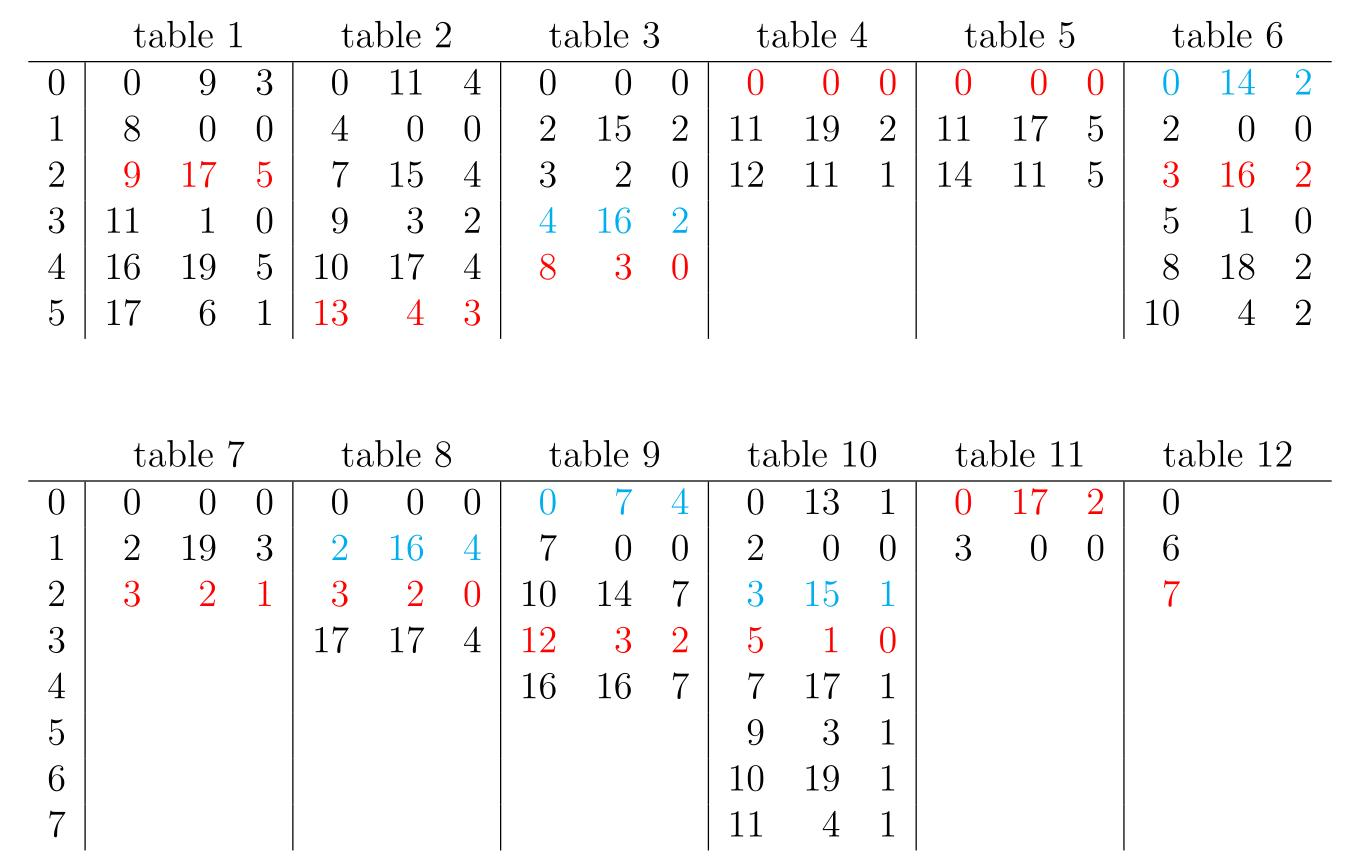
\includegraphics[width=\textwidth]{img/trick.jpg}
  \end{figure}
  Dove in rosso si hanno le varie $\pi_k(i)$ calcolate nel processo, ottenute,
  se necessario, iterando a partire dalle $\pi_k(p)$, segnalate in azzurro. \\
  Si hanno infatti i seguenti calcoli, ovvero i vari $\pi_j(i)=\pi_j(p)+i-p$,
  relativi alle permutazioni in colonna $k$ per l'estrazione della riga $9$:
  \begin{multicols}{2}
    \begin{itemize}
      \item $\pi_1(9)=17+9-9=17$
      \item $\pi_2(17)=4+17-13=8$
      \item $\pi_3(8)=4+8-8=3$
      \item $\pi_4(3)=0+3-0=3$
      \item $\pi_5(3)=0+3-0=3$
      \item $\pi_6(3)=16+3-3=16$
      \item $\pi_7(16)=2+16-3=15$
      \item $\pi_8(15)=2+15-3=14$
      \item $\pi_9(14)=3+14-12=5$
      \item $\pi_{10}(5)=1+5-5=1$
      \item $\pi_{11}(1)=17+1-0=18$
      % \item $\pi_{12}(3)=16+3-3=16$        
    \end{itemize}
  \end{multicols}
  Sfruttando quindi il valore booleano (non rappresentato nelle tabelle ma
  esistente) che ci dice con che simbolo inizia una colonna e sapendo che,
  essendo un pannello binario si alternano le run con simboli $\sigma=0$ e
  $\sigma=1$, si può ricostruire la riga 9 del pannello originale:
  \[x_9=100001000011\]
\end{esempio}
\textbf{Nel paper non si trattano metodi per effettuare query a tale struttura
  dati, indicando solo che dovrebbe essere possibile farlo.}